\documentclass[twoside]{article}
\usepackage{amsmath,amssymb,amsthm,graphicx}
\usepackage{epsfig}
\usepackage[authoryear]{natbib}

\newcommand{\reals}{\mathbf{R}}
\newcommand{\integers}{\mathbf{Z}}
\newcommand{\naturals}{\mathbf{N}}
\newcommand{\rationals}{\mathbf{Q}}

% Caligraphic alphabet
\newcommand{\calr}{\mathcal{R}} % only because \cr already taken
\newcommand{\ca}{\mathcal{A}} \newcommand{\cb}{\mathcal{B}} \newcommand{\cc}{\mathcal{C}} \newcommand{\cd}{\mathcal{D}} \newcommand{\ce}{\mathcal{E}} \newcommand{\cf}{\mathcal{F}} \newcommand{\cg}{\mathcal{G}} \newcommand{\ch}{\mathcal{H}} \newcommand{\ci}{\mathcal{I}} \newcommand{\cj}{\mathcal{J}} \newcommand{\ck}{\mathcal{K}} \newcommand{\cl}{\mathcal{L}} \newcommand{\cm}{\mathcal{M}} \newcommand{\cn}{\mathcal{N}} \newcommand{\co}{\mathcal{O}} \newcommand{\cp}{\mathcal{P}} \newcommand{\cq}{\mathcal{Q}} \newcommand{\cs}{\mathcal{S}} \newcommand{\ct}{\mathcal{T}} \newcommand{\cu}{\mathcal{U}} \newcommand{\cv}{\mathcal{V}} \newcommand{\cw}{\mathcal{W}} \newcommand{\cx}{\mathcal{X}} \newcommand{\cy}{\mathcal{Y}} \newcommand{\cz}{\mathcal{Z}}

\newcommand{\ind}[1]{1_{#1}} % Indicator function
\newcommand{\pr}{P} % Generic probability
\newcommand{\ex}{E} % Generic expectation
\newcommand{\var}{\textrm{Var}}
\newcommand{\cov}{\textrm{Cov}}
\newcommand{\sgn}{\textrm{sgn}}
\newcommand{\sign}{\textrm{sign}}
\newcommand{\kl}{\textrm{KL}} 

\newcommand{\law}{\mathcal{L}}  % \law{X}, the measure associated with r.v. X
\newcommand{\normal}{N} % for normal distribution (can probably skip this)
\newcommand{\eps}{\varepsilon}

% Convergence
\newcommand{\convd}{\stackrel{d}{\longrightarrow}} % convergence in distribution/law/measure
\newcommand{\convp}{\stackrel{P}{\longrightarrow}} % convergence in probability
\newcommand{\convas}{\stackrel{\textrm{a.s.}}{\longrightarrow}} % convergence almost surely

\newcommand{\eqd}{\stackrel{d}{=}} % equal in distribution/law/measure
\newcommand{\argmax}{\textrm{argmax}}
\newcommand{\argmin}{\textrm{argmin}}
\newcommand{\conv}{\textrm{conv}} % for denoting the convex hull

% Theorem-like declarations
\theoremstyle{plain}
\newtheorem{theorem}{Theorem}
\newtheorem{corollary}[theorem]{Corollary}
\newtheorem{lemma}[theorem]{Lemma}

\theoremstyle{definition}
\newtheorem{definition}[theorem]{Definition}
\newtheorem{example}[theorem]{Example}

\theoremstyle{remark}
\newtheorem{remark}[theorem]{Remark}



\setlength{\oddsidemargin}{0.25 in}
\setlength{\evensidemargin}{-0.25 in}
\setlength{\topmargin}{-0.6 in}
\setlength{\textwidth}{6.5 in}
\setlength{\textheight}{8.5 in}
\setlength{\headsep}{0.75 in}
\setlength{\parindent}{0 in}
\setlength{\parskip}{0.1 in}

\newcommand{\lecture}[4]{
   \pagestyle{myheadings}
   \thispagestyle{plain}
   \newpage
   \setcounter{page}{1}
   \noindent
   \begin{center}
   \framebox{
      \vbox{\vspace{2mm}
    \hbox to 6.28in { {\bf Stat210A:~Theoretical Statistics \hfill Recitation Date: #4} }
       \vspace{6mm}
       \hbox to 6.28in { {\Large \hfill #1  \hfill}  }
       \vspace{6mm}
       \hbox to 6.28in { {\it Lecturer: #2 \hfill Scribe: #3} }
      \vspace{2mm}}
   }
   \end{center}
   \markboth{#1}{#1}
   \vspace*{4mm}
}

% Local Macros Put your favorite macros here that don't appear in
% stat-macros.tex.  We can eventually incorporate them into
% stat-macros.tex if they're of general use.

\begin{document}

\lecture{Recitation 1: Probability and measure}{Tamara Broderick}{K. Jarrod
Millman \& Richard Shin}{September 3, 2014}

\section{Densities (Radon-Nikodym)}

We have a plot from the event space to values of a random variable.

\begin{figure}[ht]
  \centering
  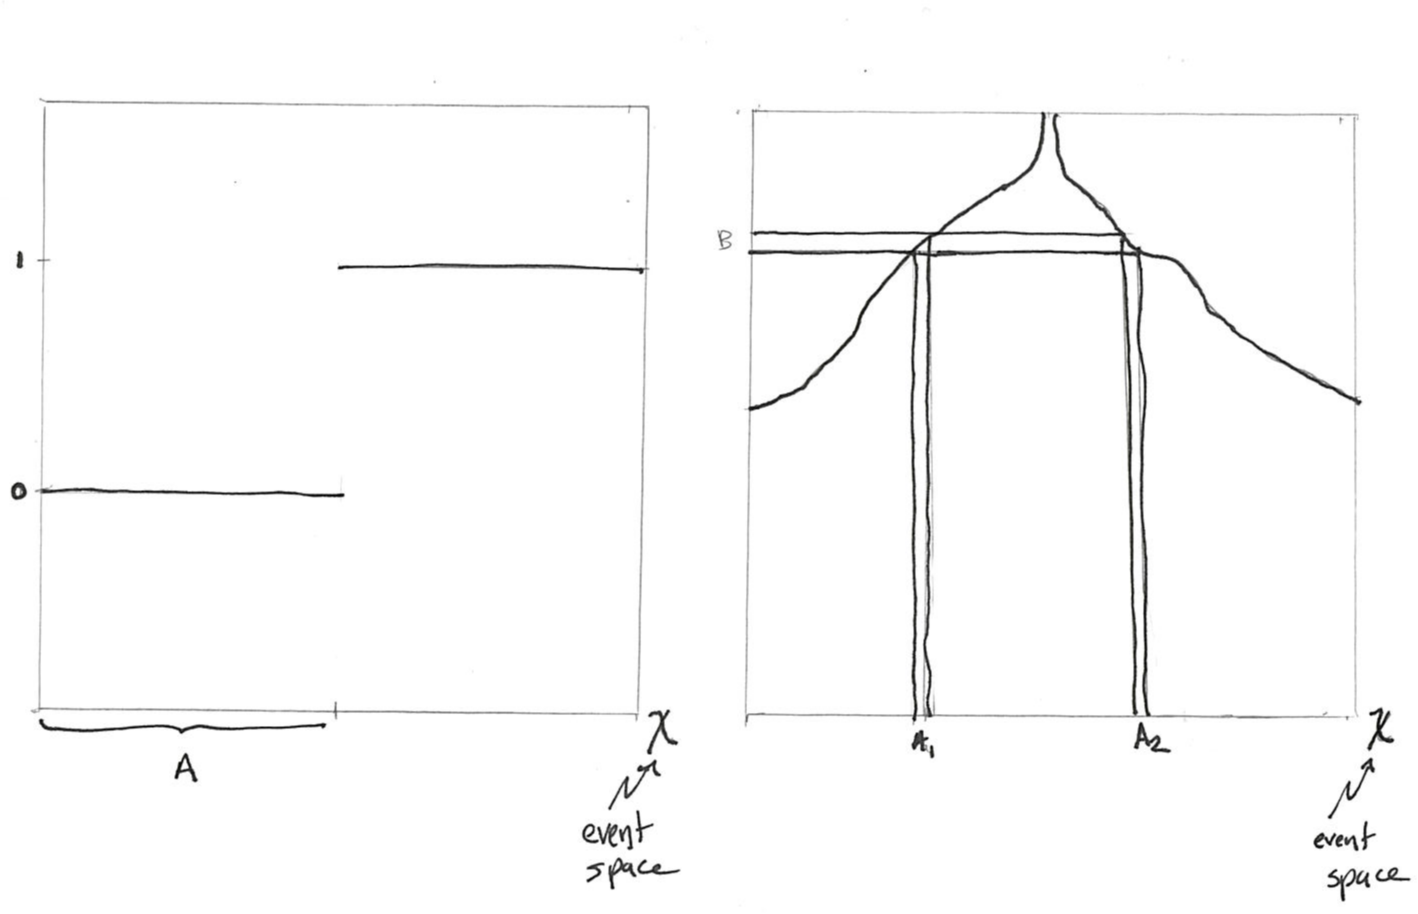
\includegraphics[width=.7\textwidth]{fig/measure-crop.pdf}
  \caption{Two frequentist risk functions where one is dominated by the other.}
  \label{fig:figure1}
\end{figure}


To compute the probability of the random variable taking on certain values
(e.g., within the interval $B$), we can measure the size of the corresponding
event space.

\begin{align*}
\mu(A = A_1 \cup A_2) \\
\nu(X \in B) &= \mu(X^{-1}(B)) = \mu(A)
\end{align*}

\begin{definition}\label{def:measure}\citep[Def. 1.4, p.~2]{keener}
  Let $\mathcal A$ be a $\sigma$-field on a set $\mathcal X$.  A real-valued function
  $\mu$ on $\mathcal A$ is called a measure if it is non-negative and countably additive:
  \begin{enumerate}
    \item  $\mu(A) \in [0, \infty]$ for all $A \in \mathcal A$.
    \item $\sum_{i=1}^\infty \mu(A_i) = \mu\left(\bigcup_{i=1}^\infty
      A_i\right)$ when $A_i$ are disjoint.
  \end{enumerate}
  We call the tuple $(\mathcal X, \mathcal A)$ a measurable space and
  $(\mathcal X, \mathcal A, \mu)$ a measure space.  If $\mu(\mathcal X) = 1$,
  $\mu$ is called a probability measure (or probability) and $(\mathcal X, \mathcal A, \mu)$
  a probablity space.
\end{definition}

In this class, we will mostly deal with the following two measures.
\begin{example} 
 If $\mathcal X = \reals^D$, let
    \[ \mu(A) = \int_{\reals^D} \cdots \int \mathbf{1}_A(x) dx_1 \cdots dx_D. \]
  Then we call $\mu$ the Lebesgue measure on $\reals^D$.
\end{example}
\begin{example} 
  If $\mathcal X$ is countable, let
    \[ \nu(A) = \#(A \cap \integers^D). \]
  Then we call $\mu$ the counting measure on $\mathcal X$.
\end{example}

It will be important to compare two measures.

\begin{definition}\label{def:absolutecontinuity}\citep[Def. 1.9, p.~7]{keener}
  Let $\mu$ and $\nu$ are be measure on a $\sigma$-field $\mathcal A$ on the
  set $\mathcal X$. Then we say that $\nu$ is absolutely continuous with respect
  to $\mu$, written $\nu \ll \mu$, if $\mu(A) = 0 \Rightarrow \nu(A) = 0$.
\end{definition}
If $\nu \ll \mu$, we also say that $\mu$ dominates $\nu$.

\begin{example}  Let $\mu$ the Lebesgue measure on $\reals$ and $\nu$ the counting
  measure on $\integers$.  Then
  \begin{align*}
    \mu(\{1\}) &= 0 \quad \nu(\{1\}) = 1 \\
    \mu((0, 1)) &= 1 \quad \nu((0, 1)) = 0
  \end{align*}
  Hence the Lebesgue measure and the counting measure are not absolutely continuous
  with respect to each other.
\end{example}

\begin{theorem}[Radon-Nikodym]\citep[Def. 1.10, p.~7]{keener}
  If a finite measure $\nu$ is absolutely continuous with respect to a
  $\sigma$-finite measure $\mu$, then there exists an essentially unique\footnote{If $h$ is
  another non-negative function that satisfies the conditions of the Radon-Nikodym theorem,
  then $h=f$ a.e. $\mu$.} non-negative function $f$
  (sometimes denoted $\frac{d\nu}{d\mu}$) such that
  \[\nu(A) = \int_A f d\mu = \int_X f \mathbf{1}_A d\mu.\]
\end{theorem}

We will often call $f$ (or $\frac{d\nu}{d\mu}$) the Radon-Nikodym density (or derivative).

\begin{example}
  If $\mu \ll \text{Lebesgue}$, then $\mu(A) = \int_A p(x) dx$.  If $\nu(A) =
  1$, then $p(x)$ is called a probability density function.
\end{example}

\begin{example}
  If $\nu$ is absolutely continuous with respect to the counting measure. Then $\nu(A)
  = \sum_{\{m\} \in A} P(m)$.  If $\nu(X) = 1$, then $p$ is a ``probability mass
  function" (e.g., Poisson).
\end{example}

For $\mu(A)$, we have
\begin{align*}
   \int \mathbf{1}_A(x) \mu(dx) &:= \mu(A) \\
   \int a \mathbf{1}_A(x) \mu(Dx) &:= \int f d\mu,\ f = a \mathbf{1}_A \\
   \int \sum_{i=1}^n a_i \mathbf{1}_{A_i}(x) \mu(dx) &:= \int f d\mu,\ f = \sum
   a_i \mathbf{1}_{A_i}
\end{align*}

\begin{definition}
  The KL divergence is
  \[ D_{KL}(\mu || \nu) = \int_\chi \log \frac{d\mu}{d\nu} d\mu \]
\end{definition}

\section{Conditional distributions (Tower Property)}

Conditional probabilities are defined as
\begin{align*}
  P(A | B) &= \frac{P(A \cap B)}{P(B)} 
\end{align*}

For discrete random variables,
\begin{align*}
  P(Y = y | X = x) = \frac{P(Y = y, X = x)}{P(X = x)}
\end{align*}

\begin{align*}
  P(Y = y) \\
  \ex[f(Y)] &= \sum_y f(y) P(Y = y) \\
  \ex[f(X, Y) | X = x] &= \sum_y f(x, y) P(Y = y | X = x)
\end{align*}
The last line is a conditional expectation.

\begin{theorem}[Tower property]
\begin{align*}
  \ex[Y | X] = \ex[\ex[Y | X, W] | X]
\end{align*}
\end{theorem}
\begin{proof}
  Here, $\ex[Y | X, W]$ is a function of $X, W$. 

  \begin{align*}
    \ex[\ex[Y | X, W] | X] &= \sum_{\tilde{x}, w} P(X = \tilde{x}, W = w | X = x)
    \cdot \left[ \sum_y yP(Y = y | X = x, W = w)\right] \\
    &= \sum_y y \sum_w \frac{P(Y = y, X = x, W = w)}{P(X = x, W = w)}  \frac{P(X =
    x, W = w)}{P(X = x)} \\
    &= \sum_y y P(Y = y | X = x)
  \end{align*}
\end{proof}
\begin{corollary}[Law of total probability]
  \[\ex[Y] = \ex[\ex[Y | W]]\]
\end{corollary}

\begin{example}
30\% of households have one child, 50\% have two children, and 20\% have
three children. What is the expected number of boys in households?
\begin{align*}
  X &= \text{\# of boys in a household} \\
  Y &= \text{\# of children in a household} \\
  \ex[X] &= \ex[\ex[X | Y]]= 0.3 \cdot 1 \cdot \frac{1}{2} + 0.5 \cdot 2 \cdot 
  \frac{1}{2} + 0.2 \cdot 3 \cdot \frac{1}{2}
\end{align*}
\end{example}

\section{Exchanging things with integration (dom. conv.)}

Our integration wish list:
\begin{itemize}
  \item $\int_t \int_x f(t, x) \mu(dx) \nu(dt) = \int_x \int_t f(t, x) \nu(dt)
    \mu(dx)$, by the Fubini-Tonelli theorem.
  \item $\lim_{n \rightarrow \infty} \int_x f_n(x) \mu(dx) = \int_x \left[
    \lim_{n \rightarrow \infty} f_n(x) \right] \mu(dx)$
  \item $\frac{\partial}{\partial t} \int_x f(t, x) \mu(dx) = \int_x
    \left[\frac{\partial}{\partial t} f(t, x)\right] \mu(dx)$
\end{itemize}

Limits are weird:
\begin{align*}
  f_n(x) &= \mathbf{1}_{(n, n+1)}(x) \\
  \lim_{n \rightarrow \infty} f_n(x) &:= 0 \\
  \lim_{n \rightarrow \infty} \int f_n(x) dx &= 1
\end{align*}

\begin{theorem}[Dominated convergence]\citep[Theorem 2.5, p.~29]{keener}
  Let ${f_n}$ be a sequence of real-valued measurable functions on a
  measure space $(\mathcal X, \mathcal A, \mu)$ such that there is some
  $g$ with $|f_n| \le g$ (a.e. $\mu$) for all $n$.  If $\int g d\mu < \infty$
  and $\lim_{n \rightarrow \infty} f_n(x) = f(x)$ for a.e. $x$ under $\mu$,
  then
  \begin{align*}
    \lim_{n \rightarrow \infty} \int f_n(x) \mu(dx) &= \int
      \left(\lim_{n \rightarrow \infty} f_n(x) \right) \mu(dx) \\
       &= \int f(x) \mu(dx) \\
       &= \int f d\mu.
  \end{align*} 
\end{theorem}

\begin{example}[from class on Tuesday]
\begin{align*}
  e^{A(\eta)} &:= \int \exp\{\eta T(x) \} h(x) \mu(dx) \\
  \eta &\in \text{canonical parameter space} \\
  \frac{\partial}{\partial \eta} e^{A(\eta)} &= e^{A(\eta)}
  \frac{\partial}{\partial \eta}A(\eta) \\
  &= \frac{\partial}{\partial \eta} \int \exp\{\eta T(x) \} h(x) \mu(dx)\\
  &= \lim_{n \rightarrow \infty} \left[ \int e^{(\eta + c/n)T(x)} h(x) \mu(dx) -
  \int e^{(\eta + 0)T(x)} h(x) \mu(dx) \right]/ \frac{c}{n} \\
  &= \lim_{n \rightarrow \infty} \int \underbrace{e^{\eta T(x)} \left[
  \frac{e^{(c/n)T(x)} - e^{0 \cdot T(x)}}{c/n} \right] h(x)}_{f_n(x)} \mu(dx) \\
  & \text{Assume $\exists g$ s.t. $|f_n(x)| \le g(x)$ and $\int g(x) \mu(dx) <
  \infty$, so dominated convergence.} \\
  &= \int \frac{\partial}{\partial \eta} \left[e^{\eta T(x)}\right] h(x) \mu(dx) \\
  &= \int T(x) e^{\eta T(x)} h(x) \mu(dx)  \\
  &= e^{A(\eta)} \ex[T(X)] \\
  &\Rightarrow \frac{\partial}{\partial \eta} A(\eta) = \ex[T(X)]
\end{align*}
\end{example}


\bibliographystyle{apalike}
\bibliography{stat}

\end{document}
